\section{System, Assumptions and Problem Formulation}
\label{sec:problemformulation}

% Background and problem model
\subsection{System and Assumptions}
\label{subsec:model}

% Background
% Multiband variation
Wireless propagation refers to the signal loss characteristics when wireless signals 
are transmitted through the wireless medium. The strength of the received signal depends on 
both the line-of-sight path (or lack thereof) and multiple other paths that result from reflection, 
diffraction, and scattering from obstacles~\cite{andersen1995propagation}. The widely-used Friis
equation characterizes the received signal power $P_r$ in terms of transmit power $P_t$, transmitter 
gain $G_t$, receiver gain $G_r$, wavelength $\lambda$ of the carrier frequency, distance $R$ from 
transmitter to receiver, and path loss exponent $n$ according to~\cite{friis}:
\begin{equation}
\label{eq:friis}
P_r=P_t+G_t+G_r+10n \log_{10}\left( \frac{\lambda}{4\pi R}\right)
\end{equation}
Here, $n$ varies according to the aforementioned environmental 
factors with a value ranging from two to five in typical outdoor 
settings~\cite{rappaport}.
% Tell the propagation of white space is much larger than wifi
Thus, the channels of low frequency white space bands propagates further than the high frequency WiFi 
bands the same RSSI threshold, transceiver settings according to Eq.~\ref{eq:friis}. 
% White spcae is good out resource to improve the service of Wifi cell
The propagation range of low frequency white space channels is times of WiFi channels, for instance, 
450 MHz channels has more than 12 times propagation range as 5 GHz channels via Friis model. Thus a 
single white space access point is possible to serve an area up to hundreds times of a WiFi access point. 
The larger propagation of white space channels is potentially to be applied for reduction of network deployment 
cost~\cite{pcuiwinmee}, adaptation of vehicular dynamic access~\cite{chen2011feasibility}, and improvement 
of network capacity~\cite{bahl2009white}.
However, previous works focus on the application of plenty white space channels resource or point to point 
communication require small amount of white space resource. 
In wireless network design, as discuss in previous works, the more wireless channel resource means the better 
performance.
Unfortunately, FCC restricts the number of white space channels in most dense populated areas due to the existing 
TV broadcasting application. Thus, a heterogeneous network with WiFi channels and few white space channels 
becomes a practical option for these cities.



% Power saving
\begin{figure}
\vspace{-0.0in}
\centering
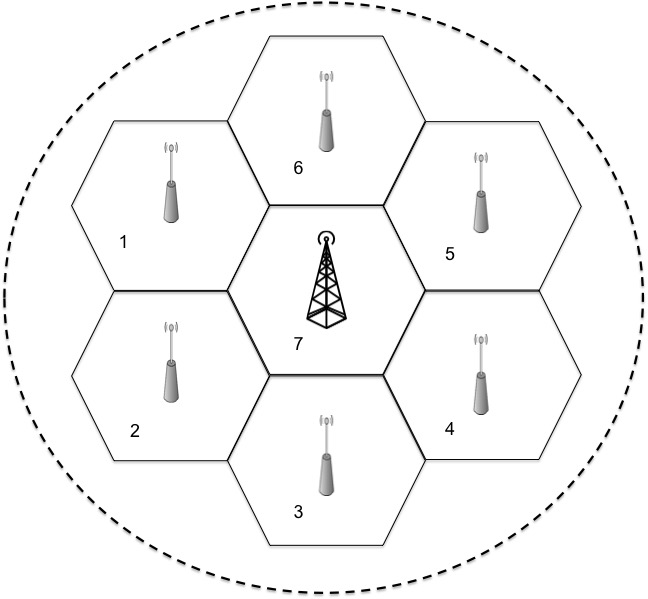
\includegraphics[width=74mm]{figures/whitecell}
\vspace{-0.1in}
\caption{White Space Model in Dense Area}
\label{fig:systemmodel}
\vspace{-0.1in}
\end{figure}


% Give the model and assumption
% B channel; N user; M AP;
Here, we introduce a heterogeneous network named as WhiteCell with existing WiFi cells and an access point 
with few number of white space channels as shown in Fig.~\ref{fig:systemmodel}.
Given a WiFi mesh wireless system with $M$ access points and $N$ users.
Each of the WiFi cell has access to the white space channels and its own WiFi channel. The reuse of 
WiFi channels has been discussed in plenty of previous works and it is out of our scope.
The users of a WiFi cell are associated with an WiFi channel assigned for the access point in the cell or one of 
the white space channels. 
There are $F_w$ white space radios is installed on one of the access points to assistant the existing WiFi 
network. 
The capacity of each radio $C$ is a equally restrict number of all the channels. There are enough buffer 
store the traffic demand from the users. 
The traffic is served in a FIFO scheduling system. 
In such a network, each user has $1+F_w$ channels to be scheduled. One is the previous in-cell WiFi channel 
and the white space channels. 
We assume the users in the same mesh cell are in a single interference domain. 
Considering the limited number of white space channels in dense area and the fact spatial reuse 
of white space will make the problem considerably more challenging, we will remains an interesting 
direction of future research. 


Instead of assuming the wireless channels are on-off~\cite{bodas2012low} or equally clean, we apply a  
measurements method to get the achieved channel capacity. The capacity of the channel between the access 
points and users is noted as a matrix in Eq.~\ref{eq:usercapacity}
\begin{equation}
\label{eq:usercapacity}
H_{i,j}^f(t)= G(\zeta,t),i \in M, j\in N, f \in (F_M+F_w) 
\end{equation} 
$\zeta$ represents the in-field measured historical data and dynamic sensing information.
We use a context-aware method to estimate the $j$ user capacity $H_{i,j}^f(t)$ to an access point 
$i$ on channel $f$. The users in a single cell has the same channel status. We assume the channel 
capacity is flat during a time slot. The switching time is negligible in the system.
The calculation of achieved channel capacity is introduced in~\ref{sec:experimentdesign}. 
The traffic demand arrive at a user as a Poisson process, with the vector noted as 
$\bm{D(t)} = [D_1(t),D_2(t),...D_N(t)]$ and the sum rate $D(t) = \sum\limits_{i=1}^N D_i(t)$. 
The rate $D(t)$ is the aggregate rate of data generated from all users. 

% Buffer and tolerance time
During a time slot, the unscheduled radios remain in sleep mode to save energy. Also we ignore 
the sleeping energy as well as the amount of energy spent on channel/radio switching. An operating 
radio will cost equal power in a time unit. Previous work~\cite{niida2010user} shows a user has a 
certain patience for waiting. The tolerance time varies across the traffic type, such as text information, 
voice information. To simply the problem, we assume an average value for $W$ of all the users in the system. 
The system applies a first-come-first-serve schedule. The white space channels are able to split for multiple 
cells.

\subsection{Problem Formulation}
\label{subsec:problem}

We formulate the system introduced in~\ref{subsec:model} as a discrete-time queuing system as shown in 
Fig.~\ref{fig:flowconfig}. 
The channels are represented as servers in the queuing system. Table.~\ref{tab:notation} 
summarizes the notation used in this work. The queuing system has $N$ queues and $F_M+F_w$ servers connecting 
by time-varying channels $H^*(N,F_M+F_w)$.


\begin{table}[htbp]
\begin{center}% used the environment to augment the vertical space
% between the caption and the table
\begin{tabular}{l l p{10cm} }
\toprule
$t$ & Time slot\\
$N$ & Set of users\\
$M$ & Set of Access points\\
$H_{ij}^f$ & Measurement based Capacity between AP i and user j on channel f\\
$F_{m}$ & WiFi Channels with Access Points\\
$F_{w}$ & Set of White Space Channels\\
$A(t)$ & User access channel schedule\\
$B$ & User Buffer\\
$C$ & Radio Capacity\\
$R$ & Operating Radio\\
$\zeta$ & In-Field Measurements\\
$W$ & Tolerance time window \\
%$R_{i}$ & $\triangleq$ & Revenue at store $i$\\
%$i$ & $\triangleq$ & index value for store locations\\
%${T}_{c}$ & $\triangleq$ & A very long description of this specific variable and is needed in the research and looks good when wrapped and aligned to the left.\\
%$TC$ & $\triangleq$ & Total overall cost(\$)\\  
%\multicolumn{3}{c}{}\\
%\multicolumn{3}{c}{\underline{Decision Variables}}\\
%\multicolumn{3}{c}{}\\
%$y_f$ & $=$ & \(\left\{\begin{array}{rl}
%1,  & \text{if Supplier located at site $f$ is open} \\
%0,  & \text{otherwise} \end{array} \right.\)\\
\bottomrule
\end{tabular}
\end{center}
\caption{Table of Notations}
\label{tab:notation}
\end{table}





\begin{figure}
\vspace{-0.0in}
\centering
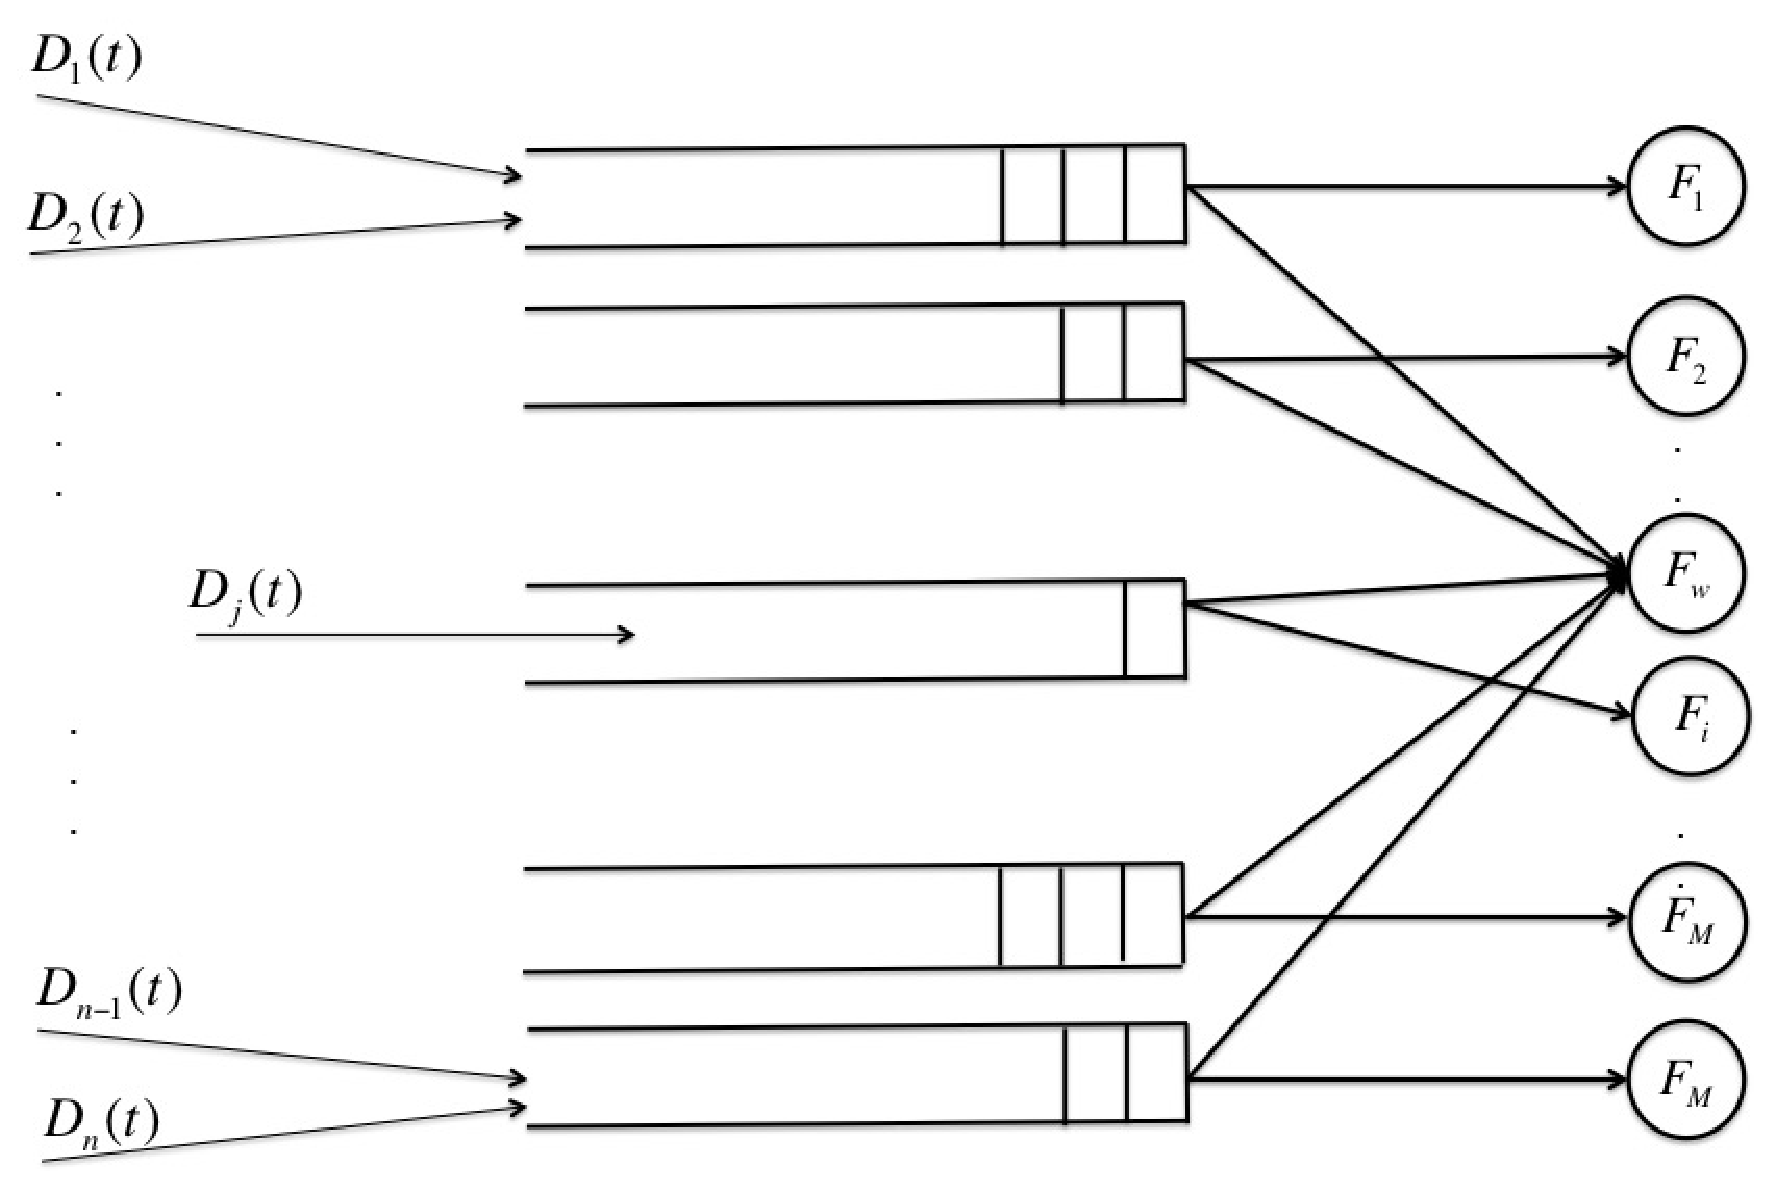
\includegraphics[width=84mm]{figures/flowconfig}
\vspace{-0.1in}
\caption{System Model}
\label{fig:flowconfig}
\vspace{-0.1in}
\end{figure}


Let matrix \{$A_{i,j}(t),i\in (F_M+F_w), j\in N$\} denote the schedule meets the 
tolerance constraint as shown in Eq.~\ref{eq:associate_def}.
%where $A_{i,j}^b = 1$ denotes user $j$ is scheduled with access point $i$ on channel $b$.
\begin{equation}
\label{eq:associate_def}
 A_{i,j}(t) = \left\{ 
	  \begin{array}{l l}
	    1   &  if\ D_{j\in N},\ is\ scheduled\ with\ \\
		& channel\ i \in (F_M+F_w) \\
		0 &  Otherwise
			    \end{array} \right.
\end{equation}

% System constraint, buffer, waiting time
%The traffic is a Poisson process, which means the users could store part of the traffic in the 
%buffer. Thus, the expected length of the queue should be less than the buffer as shown in Eq.~\ref{eq:bufferconstraint} 
%\begin{equation}
%\label{eq:bufferconstraint}
%%\sum\limits_{t^*}^{t^*+\mu_j}\gamma_j(t^*) \ge Q(t^*)+D(t^*), j\in N
%E[Q_j] \le B , j\in N
%\end{equation}
%$B$ is the buffer size of a user.

To satisfy the users, the system need to keep the expected waiting time of the system $w$ need to be less than the 
threshold $W$ as shown in Eq.~\ref{eq:timeconstraint}
\begin{equation}
\label{eq:timeconstraint}
E[w]\le W
\end{equation}


With the intuition, when the total traffic demand of the users in the system are small, one white space radio in 
white space could achieve the quality of service for the users. Thus all the WiFi radios could be turned down. 
However, as the traffic demand increase with the number of users or the demand per user, we need to increase the 
channel resource from the system to satisfy the user requirements. 
Another advantage scenario of white space channels are when some of the WiFi cells have more traffic demand, we can spend more 
white space channel capacity for these cells without building new infrastructure. 
Then the questions come as, how much power we could save through divide the white space capacity into the WiFi cells? 
And how much user traffic demand variation we could adapt in one or more cells in the system?





